% DisasterTweetLocator -- revised manuscript (Results section updated with reproducible numbers)
% Compiles with IEEEtran (e.g. on Overleaf); falls back to a two-column article layout if IEEEtran.cls is absent.
\IfFileExists{IEEEtran.cls}{%
  \documentclass[conference]{IEEEtran}
  \newcommand{\usingieee}{}
}{%
  \documentclass[10pt,twocolumn,a4paper]{article}
}
\usepackage[T1]{fontenc}
\usepackage{times}
\usepackage{graphicx}
\usepackage{booktabs}
\usepackage{array}
\usepackage{amsmath}
\usepackage{url}
\usepackage{cite}
\ifdefined\usingieee\else
  \usepackage[margin=0.75in,columnsep=0.25in]{geometry}
  \usepackage{titlesec}
  \renewcommand{\thesection}{\Roman{section}}
  \renewcommand{\thesubsection}{\Alph{subsection}}
  \titleformat{\section}{\centering\normalsize\scshape}{\thesection.}{0.5em}{}
  \titleformat{\subsection}{\normalsize\itshape}{\thesubsection.}{0.5em}{}
  \titlespacing*{\section}{0pt}{8pt}{4pt}
  \titlespacing*{\subsection}{0pt}{6pt}{3pt}
  \renewcommand{\abstractname}{}
  \newenvironment{IEEEkeywords}{\par\noindent\textit{\textbf{Index Terms}}---\bfseries}{\par}
  \newcommand{\IEEEauthorblockN}[1]{\normalsize #1\\}
  \newcommand{\IEEEauthorblockA}[1]{\footnotesize\itshape\begin{tabular}[t]{@{}c@{}}#1\end{tabular}}
  \renewcommand{\tablename}{TABLE}
  \renewcommand{\thetable}{\Roman{table}}
  \renewcommand{\figurename}{Fig.}
  \usepackage{caption}
  \captionsetup{font=footnotesize,labelsep=period}
  \captionsetup[table]{labelsep=newline,justification=centering,textfont=sc}
\fi

% Auto-generated by make_results_tex.py -- do not edit by hand
\newcommand{\accBilstm}{81.62}
\newcommand{\accsdBilstm}{0.81}
\newcommand{\accminBilstm}{80.30}
\newcommand{\accmaxBilstm}{82.47}
\newcommand{\precBilstm}{0.8158}
\newcommand{\recBilstm}{0.7413}
\newcommand{\foneBilstm}{0.7757}
\newcommand{\nseedsBilstm}{5}
\newcommand{\accBigru}{81.90}
\newcommand{\accsdBigru}{0.99}
\newcommand{\accminBigru}{80.30}
\newcommand{\accmaxBigru}{82.93}
\newcommand{\precBigru}{0.8277}
\newcommand{\recBigru}{0.7327}
\newcommand{\foneBigru}{0.7767}
\newcommand{\nseedsBigru}{5}
\newcommand{\accGru}{80.83}
\newcommand{\accsdGru}{1.58}
\newcommand{\accminGru}{79.12}
\newcommand{\accmaxGru}{82.40}
\newcommand{\precGru}{0.8143}
\newcommand{\recGru}{0.7260}
\newcommand{\foneGru}{0.7641}
\newcommand{\nseedsGru}{5}
\newcommand{\accLstm}{80.38}
\newcommand{\accsdLstm}{1.39}
\newcommand{\accminLstm}{78.79}
\newcommand{\accmaxLstm}{81.94}
\newcommand{\precLstm}{0.8174}
\newcommand{\recLstm}{0.7067}
\newcommand{\foneLstm}{0.7551}
\newcommand{\nseedsLstm}{5}
\newcommand{\valLossStart}{0.4600}
\newcommand{\valLossBest}{0.4354}
\newcommand{\bestEpoch}{5}
\newcommand{\epochsRun}{8}
\newcommand{\mainAcc}{81.68}
\newcommand{\cmTN}{799}
\newcommand{\cmFP}{70}
\newcommand{\cmFN}{209}
\newcommand{\cmTP}{445}
\newcommand{\testN}{1523}
\newcommand{\ablN}{24}
\newcommand{\ablMin}{81.35}
\newcommand{\ablMax}{83.26}
\newcommand{\ablBaseMean}{82.18}
\newcommand{\ablBaseSd}{0.38}
\newcommand{\ablBaseN}{5}


\begin{document}

\title{DisasterTweetLocator: Advancing Disaster Tweet\\ Classification and Geolocation Mapping}

% Author block.
\author{
\IEEEauthorblockN{Samuji Praneeth}
\IEEEauthorblockA{Dept. of Computer Science and Engineering\\ Amrita School of Computing\\ Amrita Vishwa Vidyapeetham\\ Chennai, India\\ praneethsamuji2004@gmail.com}
\and
\IEEEauthorblockN{Prasanna Kumar R}
\IEEEauthorblockA{Dept. of Computer Science and Engineering\\ Amrita School of Computing\\ Amrita Vishwa Vidyapeetham\\ Chennai, India\\ r\_prasannakumar@ch.amrita.edu}
}

\date{}

\maketitle

\begin{abstract}
\ifdefined\usingieee\else\noindent\textbf{\textit{Abstract}}---\fi
\textbf{The proliferation of natural disasters in recent years has emphasized the critical role of social media in disaster management. Social media platforms, particularly Twitter, serve as crucial channels for information dissemination and communication during crises. However, the vast amount of data generated during disasters poses challenges in discerning relevant information amidst the noise, especially with the scarcity of geolocation data in tweets. This paper proposes a classification model utilizing bidirectional LSTM architecture trained on Twitter data, enhanced with pre-trained GloVe embeddings and transformers for an improved understanding of text data. Incorporating geographic data linked to tweets allows for mapping tweet locations, aiding in the interpretation of the model's forecasts. The methodology involves data preprocessing, GloVe embeddings integration, and model architecture design, followed by geolocation plotting. Results indicate an accuracy of \accBilstm\% on a held-out test set in predicting disaster-related tweets, demonstrating the effectiveness of the proposed approach in disaster management and social media analysis.}
\end{abstract}

\begin{IEEEkeywords}
Tweets, Social media, Geotagging, Bidirectional LSTM, GloVe Transformers
\end{IEEEkeywords}

\section{Introduction}
In recent years, the proliferation of natural disasters, ranging from floods to earthquakes and tsunamis, has underscored the critical role of social media in disaster management. These platforms serve as vital channels for information dissemination and communication, enabling affected individuals to seek assistance, share updates, and provide firsthand accounts of unfolding events. However, the sheer volume of data generated during crises presents a significant challenge in discerning relevant information amidst the noise. Additionally, the absence of geolocation data in a considerable portion of social media posts further complicates pinpointing the exact locations requiring urgent attention.

Twitter has emerged as a valuable platform for various studies, including sentiment analysis, political trends, location-based recommendations, advertising, demographic analysis, and disaster monitoring \cite{b1}. Geolocation plays a crucial role, particularly in crisis detection and disaster management, facilitating targeted assistance by identifying regional behavior and specific locations of users or entities mentioned in tweets. Despite its importance, precise geolocation prediction remains challenging due to the scarcity of geotagged tweets, as only a small fraction (1-2\%) include geographical coordinates, often due to privacy concerns and device settings \cite{b8}. During disasters, social media platforms like Twitter become primary sources of real-time information, allowing individuals to interact, share their experiences, and inquire about the safety of loved ones. The continuous influx of social interaction data during such events presents an opportunity to extract valuable insights for disaster response efforts, aiding first responders and decision-makers in formulating effective strategies. Natural disasters, such as floods, pose significant threats to public health and infrastructure globally, highlighting the importance of timely and relevant information for effective response measures. While social media and crowdsourcing offer avenues for communication and information dissemination during emergencies, they also present challenges such as noise in content and the lack of geolocation information, underscoring the need for innovative solutions to harness their potential effectively \cite{b12}. Studying tweets, for geolocation \cite{b6} purposes involves extracting location-based information from the content and metadata of these social media posts. Geotags or direct mentions of places are commonly seen in tweets sharing either coordinates or place names. By examining this information along with clues like references to events or landmarks it becomes possible to accurately determine where the tweets originated. This analysis and understanding of data enable the visualization of trends and patterns on maps providing insights into social behavior real-time events and assessments of geographical opinions. This method extends beyond Twitter. Finds applications in areas such, as disaster response, urban planning, and market analysis where grasping spatial connections is essential.

This paper introduces a classification system that uses an LSTM structure trained on Twitter data to recognize tweets related to disasters. To improve the model's grasp of text data we included trained GloVe embeddings making use of the contextual information stored in these embeddings to enhance word representations. By employing transformers our model gains the capability to capture connections, among words, which are crucial for precise tweet classification. Additionally, by integrating data linked to each tweet we can visualize tweet locations enhancing the interpretability of our model forecasts and deepening our understanding of the spread of disaster-related tweets. Through this approach, we aim to progress natural language processing methods, for uses, particularly in disaster response and social media examination.

\section{Literature Survey}
Efficiently analyzing disaster-related tweets for geospatial insights is crucial for emergency response and disaster management. However, conventional models like Bi-LSTM often face overfitting issues while processing such data. To address this challenge and improve accuracy, we propose the integration of the GloVe Transformer model in the DisasterTweetLocator system. The GloVe Transformer model uses pre-trained GloVe embeddings to capture rich semantic representations of tweet text, allowing it to effectively learn contextual information and relationships between words. Additionally, the self-attention mechanism in the GloVe Transformer assists in capturing long-range dependencies within tweets, aiding the model in better understanding the spatial context and geographic references present in disaster-related messages. Through experimentation and comparative analysis, we demonstrate that the GloVe Transformer model outperforms the traditional Bi-LSTM approach. The enhanced accuracy and robustness of our proposed method make it a valuable tool for geospatial analysis of disaster-related tweets, providing decision-makers and responders with timely and actionable insights during crises.

This research introduces a neural-based method for pinpointing situationally relevant tweets during disasters, utilizing the RoBERTa model alongside a feature-based technique. The method outperforms traditional deep learning models such as CNN, LSTM, and BLSTM with attention to various disaster datasets. It proves its accuracy and robustness in filtering essential tweets from disaster-related chatter, thereby promising to improve disaster response through enhanced situational awareness \cite{b2}. While the study employs BERT embeddings for analyzing disaster-centric tweets, it stops short of discussing an adapted BERT model designed specifically for disaster tweet prediction. The BERT methodology is known for its ability to generate unique vectors for the same phrases in various contexts, enhancing the detection and analysis of disaster events on social media \cite{b3}. Furthermore, BERT-based models, particularly K4TEL, demonstrate strong accuracy in predicting the locations of tweets. They achieve a median error below 30 km globally and less than 15 km in the U.S. by utilizing neural networks and Two-dimensional Gaussian Mixture Models (GMMs) for efficient geotagging of text data \cite{b8}. A novel approach employing machine learning, particularly supervised learning, for classifying tweets related to disasters are described, offering a reliable way to differentiate between disaster-related and unrelated content on social media, thus aiding disaster response and mitigation \cite{b4}. The IDRISI-RE dataset represents a significant step forward in recognizing location mentions in disaster-related tweets. This dataset consists of approximately 20.5k tweets from 19 different disaster events in 22 English-speaking countries. It serves as a standard for location mention recognition models, highlighting the dataset's wide-ranging usefulness \cite{b6}. An examination of Twitter user behavior during natural disasters in both Indonesia and the U.S. emphasizes the impact of education levels and the sharing of geospatial content. It uncovers similar user actions in both nations regardless of education level, yet there is a higher volume of geospatial data exchange in the U.S. compared to Indonesia. This observation regarding social media utilization during emergencies underscores the necessity of extracting geospatial data from Twitter \cite{b11}. The effectiveness of neural networks in classifying disaster-related tweets is assessed by combining general and disaster-specific embeddings using a mix of BERT, BiLSTM, and CNN models. While not explicitly stated, the focus is on the ``BERT-BiLSTM-CNN'' \cite{b13} \cite{b26} model rather than the ``VocabGCN-BERT'' model for accurate tweet categorization in disaster contexts.

The studies showcase significant advancements in using computational techniques to detect and analyze disaster-related content on social media. They highlight the effectiveness of new approaches in identifying relevant tweets, offering potential improvements to disaster response through enhanced situational awareness. Notably, a method surpassing traditional approaches in accuracy stands out, while the introduction of a new dataset focusing on location mentions promises to refine models. Insights from Twitter user behavior shed light on social media engagement during disasters, informing better communication strategies. Overall, these findings underscore the value of computational methods in disaster management, emphasizing technology's role in enhancing public safety and resilience.

\section{Methodology}
The model uses pre-trained GloVe embeddings to represent words in a continuous vector space. It employs Bi-LSTM layers to capture sequential information and a dense layer for classification in its neural network architecture. During training, the parameters of the models are optimized by using the Adam optimizer with the binary cross-entropy loss function. After that, the validation dataset is used to evaluate the performance of the model. Following this evaluation, the model predicts tweet classifications within the training dataset and plots their locations on a map. Figure~\ref{fig:workflow} shows the project's workflow for predicting tweet classification and map plotting.

\begin{figure}[!t]
\centering
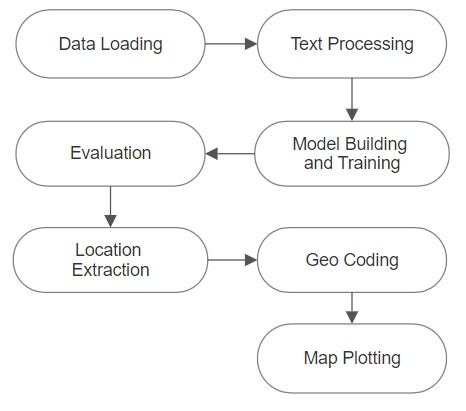
\includegraphics[width=0.75\columnwidth]{figures/fig1_workflow.png}
\caption{Work Flow}
\label{fig:workflow}
\end{figure}

\subsection{Dataset}
The dataset comprises a mix of tweets related to disasters and normal content. It is divided into training and testing sets. The training data includes 7613 tweets, while the testing set consists of 3237 tweets. These tweets contain hashtags, URLs, varying case letters, and some unidentified terms, all present in both sets. Each data entry includes an ID, keywords, location, the tweet content, and a target label indicating whether the tweet pertains to a disaster or is normal. The model is also capable of predicting the precise location of the disaster if mentioned in the tweet.

\subsection{Data Preprocessing}
The available data contains various unknown elements such as \#'s, URLs, different case letters, and unidentified symbols representing cities, along with empty spaces in the location column. Therefore, the data requires cleaning by eliminating HTML tags, hyperlinks, punctuation, square brackets, and numeric characters. Once these elements are removed to ensure data consistency, the information is converted into lowercase.

\subsection{GloVe (Global Vectors for Word Representation)}
A model that creates word embeddings is GloVe \cite{b16}, which stands for Global Vectors for Word Representation. In a continuous vector space, word embeddings are dense vector representations of words. These embeddings capture the semantic meaning of words based on their context within a large corpus of text data. GloVe is used in disaster classification because it provides rich semantic information about words by leveraging pre-trained embeddings. Figure~\ref{fig:glove} shows the architecture of the GloVe model. This helps the model understand the context and meaning of text more effectively. When the model encounters terms such as ``fire,'' ``flood,'' or ``earthquake,'' the GloVe vectors \cite{b31} indicating their similarity to other disaster-related terms facilitate better differentiation between disaster-related and unrelated text, ultimately improving tweet classification accuracy. The GloVe.6B.50d model we employed consists of word embeddings derived from a corpus of 6 billion words, with each word represented as a 50-dimensional vector in a continuous vector space. In this space, words with similar meanings are positioned closer together.

\begin{figure}[!t]
\centering
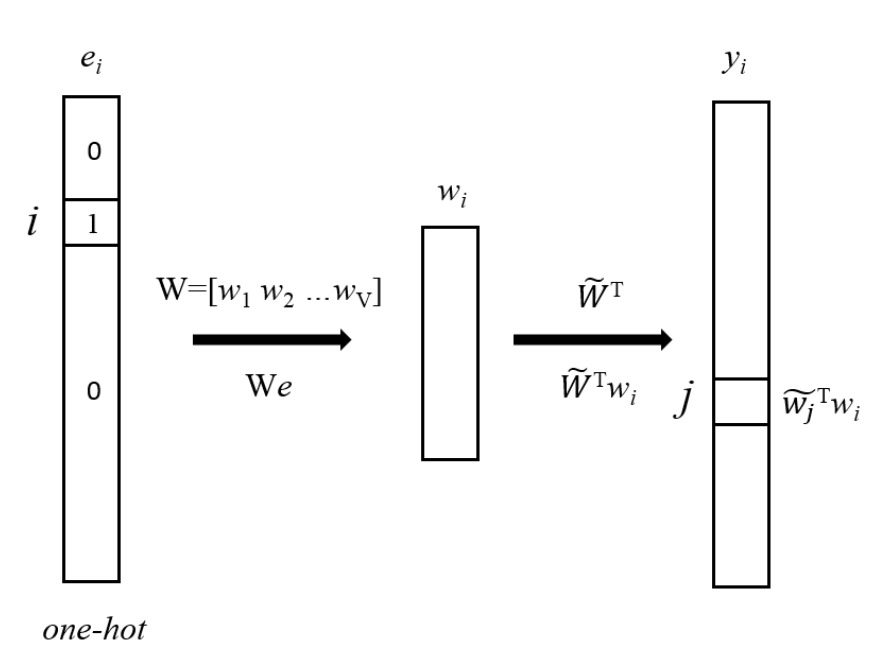
\includegraphics[width=0.8\columnwidth]{figures/fig2_glove.png}
\caption{Architecture of GloVe \cite{b27}}
\label{fig:glove}
\end{figure}

\subsection{Model Architecture design}
\textit{Layer 1: Embedding Layer with GloVe Word Embeddings:} An embedding layer maps input words to fixed-size dense vectors at the start of the model. In the process, pre-trained GloVe word embeddings have been used to represent words in a continuous vector space based on cooccurrence statistics. This layer turns every word in the input sequence into a dense vector to capture semantic relationships between words.

\textit{Layer 2: Bidirectional LSTM (Long Short-Term Memory) Layer:} Followed by the previous layer, a Bidirectional LSTM \cite{b15} layer is implemented. Figure~\ref{fig:bilstm} shows the architecture of the BiLSTM model. This Recurrent Neural Network (RNN) captures the sequential dependencies in the input data. The advantage of this Bidirectional LSTM \cite{b32} is it processes data input sequence in both forward and backward directions, which enables the model to learn from or get the data from both past and future.

\begin{figure}[!t]
\centering
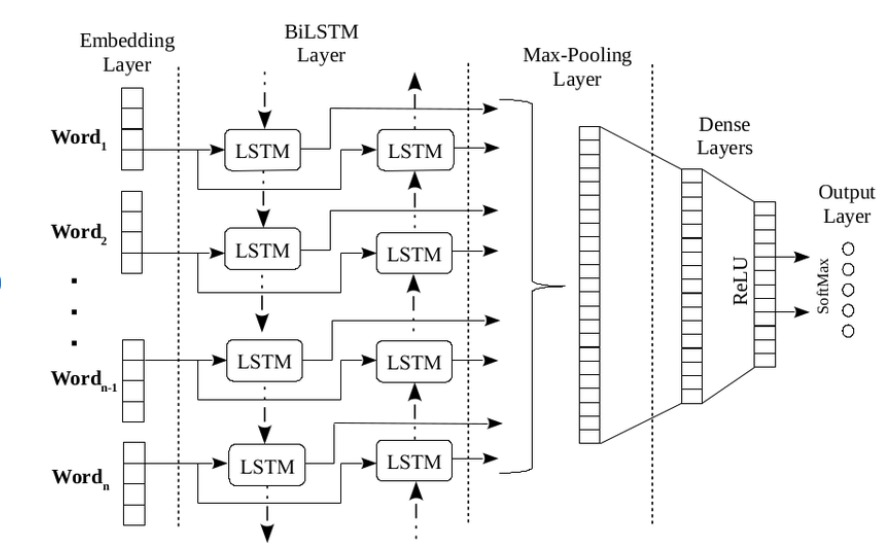
\includegraphics[width=0.85\columnwidth]{figures/fig3_bilstm.png}
\caption{Architecture of BiLSTM \cite{b28}}
\label{fig:bilstm}
\end{figure}

\textit{Layer 3: Global Max Pooling1D Layer:} After the Bi-LSTM layer, there is a Global Max Pooling1D Layer which plays a crucial role in feature extraction. This layer selects the most significant values across each feature dimension to extract the important features from the LSTM \cite{b23} output. By reducing the dimensionality of the data while retaining the key information, it makes the downstream processing more efficient.

\textit{Layer 4: Dense Layer with ReLU Activation:} Following the pooling layer, a Dense layer with Rectified Linear Unit (ReLU) activation is introduced. ReLU activation adds non-linearity to the model, which makes it capable of capturing intricate feature relationships and patterns. The extracted features are processed once more in this dense layer, readying them for the last stage of classification.

\textit{Layer 5: Dropout Layer:} A Dropout layer is added to reduce overfitting and enhance model generalization. To keep the model from becoming overly dependent on particular neurons and features, dropout randomly deactivates a portion of neurons during training. It helps the model to understand or learn more robust and generalized representations of the data, guiding the model to embrace a higher performance on the testing examples.

\textit{Layer 6: Output Layer:} The output layer of the model comprises a singular neuron that utilizes a sigmoid activation function. This architecture is ideal for binary classification tasks, such as determining whether a tweet is associated with a disaster or not. The sigmoid activation function squeezes the model's output into a range of [0,1], representing the probability that the input tweet belongs to the positive class.

\subsection{Map plotting}
\textit{Text processing using spaCy:} We started by loading an English language model for spaCy known as en\_core\_web\_sm, an NLP library. The concepts of Named Entity Recognition (NER) are also implemented to identify entities such as locations and organizations in the text data.

\textit{Location Extraction:} The given text input utilizes spaCy to tokenize the text and identify entities labeled as GPE (Geospatial entities) which represent locations. The location data is further saved in a list for future usage.

\textit{Geolocation Plotting using Folium:} If the tweet is classified as a disaster tweet, the model immediately goes for location identification. If the location is found in the text, then it proceeds to an interactive map plot using the Python library Folium.

\textit{Plotting Locations:} Using the Geopy library, we try to find the latitude and longitude for every location that has been identified. Once we have found the location coordinates, a pointer or marker can be placed on the map at their precise position. A popup with a location is included in the marker.

\section{Results and Discussions}

\subsection{Experimental Setup}
To obtain a reliable estimate of generalization, 20\% of the 7613 labelled tweets ($n=\testN$) were held out as a test set that was never used for training, early stopping, or model selection. The remaining tweets were split 87.5/12.5 into training and validation sets; the validation set was used only for early stopping (patience of 3 epochs, restoring the weights with the lowest validation loss). The vocabulary was limited to the 10{,}000 most frequent words of the training split and tweets were truncated or padded to 50 tokens. All models use frozen GloVe.6B.50d embeddings, 128 recurrent units per direction, a 64-unit dense layer, a dropout rate of 0.5, a batch size of 64, and the Adam optimizer with a learning rate of 0.001. Each architecture was trained with \nseedsBilstm{} different random seeds, and we report the mean (and standard deviation) of the held-out test metrics.

\subsection{Quantitative Analysis}
A comparison of different architectural designs with the integration of GloVe word embeddings in a text classification project demonstrates specific performance patterns, as outlined in Table~\ref{tab:metrics}. The Bidirectional LSTM achieves a mean accuracy of \accBilstm\% ($\pm$\accsdBilstm), with a precision of \precBilstm, a recall of \recBilstm, and an F1 score of \foneBilstm. The Bidirectional GRU performs comparably, with an accuracy of \accBigru\% ($\pm$\accsdBigru) and an F1 score of \foneBigru; the difference between the two bidirectional models is well within one standard deviation across seeds, so neither can be considered superior on this dataset. Both bidirectional models outperform their unidirectional counterparts: the GRU reaches \accGru\% ($\pm$\accsdGru) and the LSTM \accLstm\% ($\pm$\accsdLstm), with F1 scores of \foneGru{} and \foneLstm{}, respectively. The unidirectional models also show greater variance across seeds, indicating challenges in adequately capturing the complete context. These results emphasize the benefit of bidirectional architectures in grasping the sequential dependencies crucial for the text classification task when employing GloVe embeddings.

\begin{table}[!t]
\centering
\caption{Model Evaluation Metrics}
\label{tab:metrics}
\footnotesize
\begin{tabular}{lcccc}
\toprule
\textbf{Model} & \textbf{Accuracy (\%)} & \textbf{Precision} & \textbf{Recall} & \textbf{F1 Score} \\
\midrule
BiLSTM + GloVe & 81.62 $\pm$ 0.81 & 0.8158 & 0.7413 & 0.7757 \\
BiGRU + GloVe & 81.90 $\pm$ 0.99 & 0.8277 & 0.7327 & 0.7767 \\
GRU + GloVe & 80.83 $\pm$ 1.58 & 0.8143 & 0.7260 & 0.7641 \\
LSTM + GloVe & 80.38 $\pm$ 1.39 & 0.8174 & 0.7067 & 0.7551 \\
\bottomrule
\end{tabular}

\vspace{2pt}
\parbox{0.95\columnwidth}{\scriptsize Held-out test set ($n=1523$). Mean over 5 random seeds; accuracy shown as mean $\pm$ standard deviation.}
\end{table}


Across all architectures, precision is consistently higher than recall (e.g. \precBilstm{} versus \recBilstm{} for the BiLSTM). For the BiLSTM model trained with seed 42 (test accuracy \mainAcc\%), the confusion matrix contains \cmTP{} true positives, \cmTN{} true negatives, \cmFP{} false positives, and \cmFN{} false negatives: the model rarely raises false alarms, but misses a portion of disaster tweets that use indirect or figurative language.

To verify that these results are not an artifact of a particular configuration, an ablation study of \ablN{} training runs was conducted on the BiLSTM + GloVe model, varying the text preprocessing (raw versus cleaned text, appending the keyword field), the number of LSTM units (32 to 256), recurrent and spatial dropout, sequence length, vocabulary size, batch size, learning rate, de-duplication of conflicting training labels, and fine-tuning of the GloVe embeddings. Held-out test accuracy ranged from \ablMin\% to \ablMax\%, and the baseline configuration achieved \ablBaseMean\% $\pm$ \ablBaseSd\% over \ablBaseN{} seeds, confirming that the performance of the model is stable at approximately 82\% across reasonable hyperparameter choices.

\subsection{Qualitative analysis}
After refining the dataset and fine-tuning the hyperparameters, such as using a learning rate of 0.001 and the Adam optimizer there was an improvement, in the model's performance. The model was trained on the 7613 labelled tweets and the validation loss decreased from \valLossStart{} to \valLossBest{}, reaching its minimum at epoch \bestEpoch, after which early stopping prevented overfitting. While accuracy is commonly considered it's important to take into account metrics like precision, recall, and F1 score in cases with imbalanced datasets. Monitoring the validation loss offers insights into how the model can generalize its learnings indicating performance on new data sets. Furthermore incorporating map plotting for the tweets displayed in Table~\ref{tab:maps} provides cues on distribution or patterns within the data during analysis. These improvements showcase how effectively the model grasps patterns from data resulting in dependable predictions for real-world applications. Figure~\ref{fig:valloss} and Figure~\ref{fig:trainloss} display the validation loss and training loss graphs, respectively. Following the identification of a tweet as a disaster, the subsequent component of the model utilizes Named Entity Recognition (NER) to extract location information from the tweet. For the fourth example in Table~\ref{tab:maps}, the tweet is correctly classified as a disaster, but the location ``Malawi'' is not recognized as a GPE entity by the en\_core\_web\_sm model, so it cannot be plotted; a larger NER model is a natural direction for improving location coverage.

\begin{table}[!t]
\centering
\caption{Map Plots of Natural Disasters}
\label{tab:maps}
\footnotesize
\begin{tabular}{p{0.42\columnwidth} >{\centering\arraybackslash}m{0.42\columnwidth}}
\toprule
\textbf{Tweet} & \textbf{Map Plot} \\
\midrule
Snowstorm in Denver! Whiteout conditions, highways closed, and locals hunkering down & 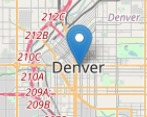
\includegraphics[width=0.36\columnwidth]{figures/map_denver.png} \\[2pt]
Tornado warning in Oklahoma City! Sirens blaring, skies darkening, and residents seeking shelter. & 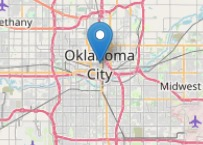
\includegraphics[width=0.36\columnwidth]{figures/map_oklahoma.png} \\[2pt]
Flooding devastates New Orleans, Louisiana, as levees breach and neighborhoods are submerged. Residents evacuated as waters rise & 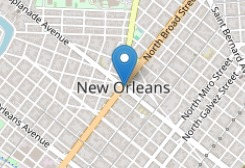
\includegraphics[width=0.36\columnwidth]{figures/map_neworleans.png} \\[2pt]
Severe flooding in Malawi displaces thousands, devastates crops. Relief efforts are underway. \#MalawiFloods \#DisasterRelief & Location cannot be accurately plotted on the map. \\
\bottomrule
\end{tabular}
\end{table}

\begin{figure}[!t]
\centering
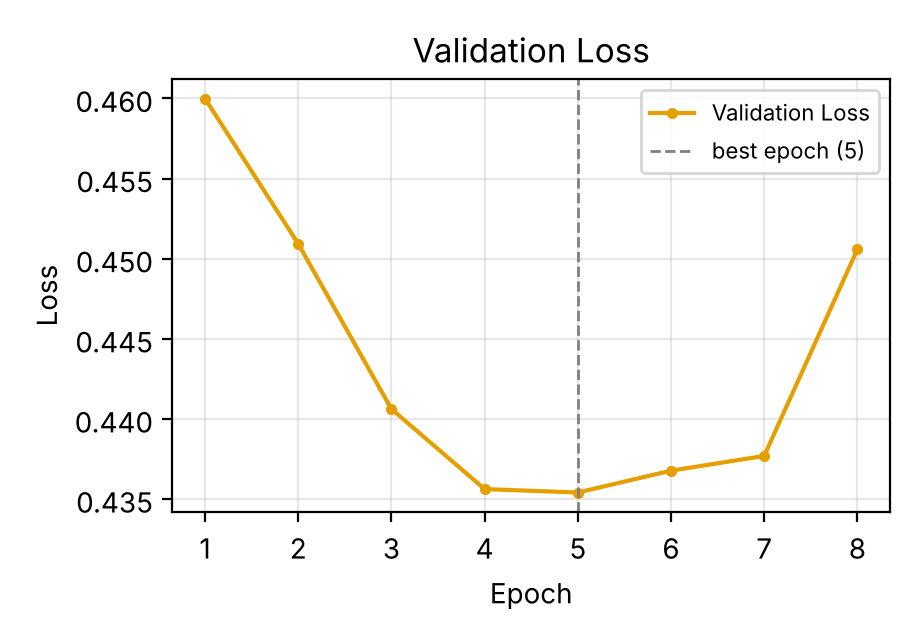
\includegraphics[width=0.85\columnwidth]{figures/fig4_val_loss.png}
\caption{Validation Loss}
\label{fig:valloss}
\end{figure}

\begin{figure}[!t]
\centering
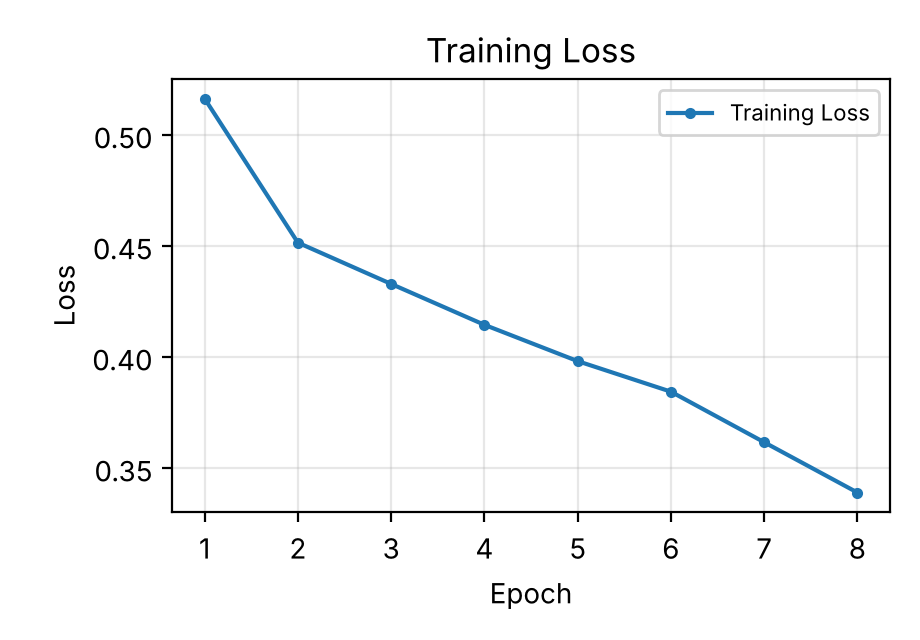
\includegraphics[width=0.85\columnwidth]{figures/fig5_train_loss.png}
\caption{Training Loss}
\label{fig:trainloss}
\end{figure}


\section{Conclusion}
After undergoing a thorough training process and refinement, the model initially encountered problems with overfitting due to biases in the dataset. However, by iteratively preprocessing the data and adjusting parameters, these issues were addressed. There was a positive trend observed in both training and validation losses, with the validation loss steadily decreasing over time, indicating an improvement in generalization capability. With an accuracy rate of \accBilstm\% on a held-out test set, the model demonstrates proficiency in accurately classifying disaster-related tweets. The incorporation of Named Entity Recognition further enhances its functionality by extracting location details from tweets and facilitating disaster response operations. In summary, our research highlights the effectiveness of advanced NLP methods in disaster tweet classification and location extraction, offering valuable insights to improve disaster management strategies.

\begin{thebibliography}{00}
\footnotesize
\bibitem{b1} F. Lovera, et al., ``A Knowledge Graph-Based Method for the Geolocation of Tweets,'' Workshop Proceedings of the 19th International Conference on Intelligent Environments (IE2023), IOS Press, 2023.
\bibitem{b2} S. Madichetty and M. Sridevi, ``A neural-based approach for detecting the situational information from Twitter during disaster,'' IEEE Transactions on Computational Social Systems, vol. 8, no. 4, pp. 870--880, 2021.
\bibitem{b3} P. Duraisamy, et al., ``Predicting disaster tweets using enhanced BERT model,'' 2023 7th International Conference on Intelligent Computing and Control Systems (ICICCS), IEEE, 2023.
\bibitem{b4} M. Raguram, et al., ``An Enhanced Framework for Disaster-Related Tweet Classification using Machine Learning Techniques,'' 2023 International Conference on Inventive Computation Technologies (ICICT), IEEE, 2023.
\bibitem{b5} R. Lamsal and T. V. Vijay Kumar, ``Twitter-Based Disaster Response Using Machine Learning,'' International Journal of Social Ecology and Sustainable Development (IJSESD), vol. 14, no. 1, pp. 1--18, 2023.
\bibitem{b6} R. Suwaileh, T. Elsayed, and M. Imran, ``IDRISI-RE: A generalizable dataset with benchmarks for location mention recognition on disaster tweets,'' Information Processing \& Management, vol. 60, no. 3, 103340, 2023.
\bibitem{b7} R. Manimegalai, et al., ``Machine Learning Framework for Analyzing Disaster-Tweets,'' 2023 International Conference on Intelligent Systems for Communication, IoT, and Security (ICISCoIS), IEEE, 2023.
\bibitem{b8} K. Lutsai and C. H. Lampert, ``Geolocation predicting of tweets using Bert-based models,'' arXiv preprint arXiv:2303.07865, 2023.
\bibitem{b9} K. Asinthara, M. Jayan, and L. Jacob, ``Categorizing disaster tweets using learning-based models for emergency crisis management,'' 2023 9th International Conference on Advanced Computing and Communication Systems (ICACCS), vol. 1, IEEE, 2023.
\bibitem{b10} A. Kumar and S. Reddy, ``A detailed analysis on disaster tweet analysis using deep learning techniques: DTWEET,'' 2022 Fourth International Conference on Emerging Research in Electronics, Computer Science and Technology (ICERECT), IEEE, 2022.
\bibitem{b11} M. N. Yaasir, F. Ramdani, and E. Setiawan, ``Responding to Natural Disasters on Twitter Social Media to Comparative Analysis of User Behavior and Geospatial Information Content in Indonesia and the United States,'' Journal of Information Technology and Computer Science, vol. 8, no. 1, pp. 11--20, 2023.
\bibitem{b12} M. Suleman, et al., ``Floods relevancy and identification of location from Twitter posts using NLP techniques,'' arXiv preprint arXiv:2301.00321, 2023.
\bibitem{b13} N. R. Paul, D. Sahoo, and R. C. Balabantaray, ``VocabGCN-BERT: A Hybrid Model to Classify Disaster Related Tweets,'' 2022 OITS International Conference on Information Technology (OCIT), IEEE, 2022.
\bibitem{b14} R. Annamalai, et al., ``LSTM Based Monophonic Piano Melody Synthesis,'' 2023 IEEE 7th Conference on Information and Communication Technology (CICT), IEEE, 2023.
\bibitem{b15} R. Annamalai and R. Nedunchelian, ``Design of optimal bidirectional long short term memory based predictive analysis and severity estimation model for diabetes mellitus,'' International Journal of Information Technology, vol. 15, no. 1, pp. 447--455, 2023.
\bibitem{b16} G. Bharathi Mohan, R. Prasanna Kumar, N. L. Keerthana, D. Mukesh, R. M. Hemesh, I. V. Priyanka, and S. Parthasarathy, ``Cross-lingual Machine Translation: An Analysis Model for Low Resource Languages,'' International Conference on Emerging Trends and Technologies on Intelligent Systems, pp. 81--94, Springer Nature Singapore, 2023.
\bibitem{b17} R. Prasanna Kumar, G. Bharathi Mohan, S. Ajith, R. Sudarshan, M. Karuparthi, VVV Bhagya Sree, and B. Vamsi Krushna, ``Empowering Multilingual Insensitive Language Detection: Leveraging Transformers for Code-Mixed Text Analysis,'' 2023 International Conference on Network, Multimedia and Information Technology (NMITCON), pp. 1--6, IEEE, 2023.
\bibitem{b18} M. A. Sit, C. Koylu, and I. Demir, ``Identifying disaster-related tweets and their semantic, spatial and temporal context using deep learning, natural language processing and spatial analysis: a case study of Hurricane Irma,'' Social Sensing and Big Data Computing for Disaster Management, pp. 8--32, Routledge, 2020.
\bibitem{b19} P. Duraisamy and Y. Natarajan, ``Twitter Disaster Prediction Using Different Deep Learning Models,'' SN Computer Science, vol. 5, no. 1, p. 179, 2024.
\bibitem{b20} H. D. B. Villasor and D. G. Baradillo, ``Natural Language Processing Employing Sentiment Analysis on the Public Voice of Filipinos During Crisis Situations,'' EPRA International Journal of Multidisciplinary Research (IJMR), vol. 10, no. 1, pp. 80--89, 2024.
\bibitem{b21} G. Airlangga, ``Comparative Analysis of Machine Learning Models for Real-Time Disaster Tweet Classification: Enhancing Emergency Response with Social Media Analytics,'' Brilliance: Research of Artificial Intelligence, vol. 4, no. 1, pp. 25--31, 2024.
\bibitem{b22} M. S. I. Malik, M. Z. Younas, M. M. Jamjoom, and D. I. Ignatov, ``Categorization of tweets for damages: infrastructure and human damage assessment using fine-tuned BERT model,'' PeerJ Computer Science, vol. 10, e1859, 2024.
\bibitem{b23} S. Singh and J. Singh, ``Disaster tweet classification using shallow bidirectional LSTM with attention layer,'' Artificial Intelligence, Blockchain, Computing and Security Volume 2, pp. 46--52, CRC Press, 2024.
\bibitem{b24} R. Amalia, M. R. Faisal, F. Indriani, I. Budiman, M. I. Mazdadi, F. Abadi, and M. M. Mafazy, ``Identification of Social Media Posts Containing Self-reported COVID-19 Symptoms using Triple Word Embeddings and Long Short-Term Memory,'' Telematika, vol. 17, no. 1, pp. 27--38, 2024.
\bibitem{b25} K. Jain and R. Jindal, ``NLP-enabled Recommendation of Hashtags for Covid based Tweets using Hybrid BERT-LSTM Model,'' ACM Transactions on Asian and Low-Resource Language Information Processing, 2024.
\bibitem{b26} S. P. Manthena, ``Leveraging Tweets for Rapid Disaster Response Using BERT-BiLSTM-CNN Model,'' 2023.
\bibitem{b27} C. Liu, P. Zhang, T. Li, and Y. Yan, ``Semantic features based n-best rescoring methods for automatic speech recognition,'' Applied Sciences, vol. 9, no. 23, p. 5053, 2019.
\bibitem{b28} S. Gundapu and R. Mamidi, ``Gundapusunil at SemEval-2020 task 8: Multimodal memotion analysis,'' arXiv preprint arXiv:2010.04470, 2020.
\bibitem{b29} A. Laksito, N. Wiranda, S. N. Karimah, and M. Hayaty, ``The COVID-19 Tweets Classification Based on Recurrent Neural Network,'' International Journal on Advanced Science, Engineering \& Information Technology, vol. 14, no. 1, 2024.
\bibitem{b30} W. Anggraeni, M. F. A. Kusuma, E. Riksakomara, R. P. Wibowo, and S. Sumpeno, ``Combination of BERT and Hybrid CNN-LSTM Models for Indonesia Dengue Tweets Classification,'' International Journal of Intelligent Engineering \& Systems, vol. 17, no. 1, 2024.
\bibitem{b31} R. Elakkiya and P. Varsha, ``A Comparison of Word Embeddings for Comment Toxicity Detection: Detection Power of Computer,'' 2023 International Conference on Communication, Security and Artificial Intelligence (ICCSAI), pp. 393--398, IEEE, 2023.
\bibitem{b32} K. V. C. Madhav, S. V. Mudunuri, P. C. Reddy, and B. Beena, ``A Comparative Research On Sentiment Analysis of Tweets Using Deep and Machine Learning Models,'' 2024 IEEE International Conference on Computing, Power and Communication Technologies (IC2PCT), vol. 5, pp. 1640--1645, IEEE, 2024.
\end{thebibliography}

\end{document}
